\section{Introduksjon}
Det er ingen hemmelighet at det festes mye gjennom studietiden og som konsekvens fører dette til at noen velger å fyllekjøre, enten om det er for å komme seg hjemm eller for å ta med festen på veien. Samtidig er det ingen god løsning til dette problemet, selv om loven straffer hardt mot fyllekjøring hindrer det ikke noen prøver seg. Så hvordan kan dette begrenses?

Lille Promille er en app som takler dette problemet ved å fokusere på selve drikkingen. Hvis man kan kontrollere seg selv og sine venner, vil man kunne ta bedre valg og unngå å kjøre i påvirket tilstand. For å gjøre dette, tilbyr appen en oversikt over kjøretilstanden sin. Man får innsikt til alkohol i blodet, antall drikker man har drukket, og hvor lenge det er til man kan kjøre bil. Det vil også være et vennesystem der man kan se hvor mye venner har drukket, som bidrar i å engasjere studenter til å bruke appen.

Appen vil ikke kun være for studenter, men alle som ønsker å ha kontroll mens man fester. Visjonen er at man kommer til å bruke Lille Promille appen for å få oversikt over hvor man drikker, samt hvor mye venner drikker. Det vil være en app som gjør festingen bedre men samtidig minsker sjansen for fyllekjøring, siden dette er av erfaring noe mange lurer på mens de er påvirket.

\subsection{Hvordan fungerer appen?}
\subsubsection{Et eksempel}
Ta utgangspunkt i at det er en fest på en søndagskveld, og dagen etter må man være klar til å kjøre til høgskolen tidlig ettermiddagen. Når man tar sin første drikk, åpner man appen og legger til en enhet som passer drikken, for eksempel en rusbrus. Man velger å legge til disse for hver slurk eller for hver flaske man har drukket. Appen vil med jevne mellomrom beregne promillen, slik at man har full oversikt gjennom hele festen. Appen viser rett før midnatt at det er tolv timer til man er kjørbar, og man velger å stoppe å drikke.

Dagen derpå sjekker man appen og ser at det fremdeles er noen venner som er påvirket, og til og med noen som enda drikker. Men siden man følgte appens anvisninger, er man sikrere på at man har beholdt promillegrensen og er klar til å kjøre bil. I tillegg har man muligheten til å se hvordan økten gikk på festen, som hvor man befant seg til diverse tider, hvor mye man drakk og hvor ofte. Disse dataene kan man igjen bruke til senere fester slik at man blir sikrere på sine egne grenser og hva man tåler av alkohol.

\subsubsection{Flytdiagram}

\begin{figure}[H]
    \centering
    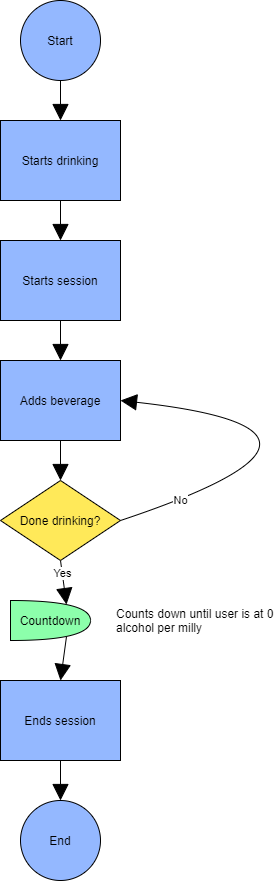
\includegraphics[scale=0.4]{images/lille_promille_user_float.drawio.png}
    \caption{Diagram som viser hvordan bruker vanligvis vil samhandle med appen.}
\end{figure}